% !TEX TS-program = pdflatex
% !TEX encoding = UTF-8 Unicode

% This is a simple template for a LaTeX document using the "article" class.
% See "book", "report", "letter" for other types of document.

\documentclass[11pt]{article} % use larger type; default would be 10pt

\usepackage[utf8]{inputenc} % set input encoding (not needed with XeLaTeX)

%%% Examples of Article customizations
% These packages are optional, depending whether you want the features they provide.
% See the LaTeX Companion or other references for full information.

%%% PAGE DIMENSIONS
\usepackage{geometry} % to change the page dimensions
\geometry{letterpaper} % or letterpaper (US) or a5paper or....
\geometry{margin=1in} % for example, change the margins to 2 inches all round
% \geometry{landscape} % set up the page for landscape
%   read geometry.pdf for detailed page layout information

\usepackage{graphicx} % support the \includegraphics command and options
\usepackage{hyperref}

\usepackage[parfill]{parskip} % Activate to begin paragraphs with an empty line rather than an indent

%%% PACKAGES
%\usepackage{booktabs} % for much better looking tables
\usepackage{array} % for better arrays (eg matrices) in maths
%\usepackage{paralist} % very flexible & customisable lists (eg. enumerate/itemize, etc.)
\usepackage{verbatim} % adds environment for commenting out blocks of text & for better verbatim
%\usepackage{subfig} % make it possible to include more than one captioned figure/table in a single float
% These packages are all incorporated in the memoir class to one degree or another...

%%% HEADERS & FOOTERS
\usepackage{fancyhdr} % This should be set AFTER setting up the page geometry
\pagestyle{fancy} % options: empty , plain , fancy
\renewcommand{\headrulewidth}{0pt} % customise the layout...
\lhead{}\chead{}\rhead{}
\lfoot{}\cfoot{\thepage}\rfoot{}

%%% END Article customizations

%%% The "real" document content comes below...

\title{The Power to Control}
\author{Advanced Arduino Workshop}
\date{} % Activate to display a given date or no date (if empty),
         % otherwise the current date is printed 

\begin{document}
\maketitle

%\begin{quote}
%Wise quote here.\\ \hbox{}\hfil -- {\em A Wise One}
%\end{quote}

\section*{Updates for next time}

\begin{itemize}
    \item Instructions on using a DMM
    \item Appendix on HEX
    \item Pre-lab needs to have them come with laser checker, which needs better instruction in comparison to button
    \item Make it easier to turn in places where they recorded values?
\end{itemize}
\section*{Introduction}

In previous tutorials, you've been introduced to Arduino, an accessible prototyping platform for electromechanical systems. Those tutorials focused on the basic functionality of Arduino -- methods used to connect and read sensors or control an LED or motor. In this workshop, we'll focus on techniques for building more complex programs -- programs that have to perform more than one or two tasks.

When programming a microcontroller to perform a set of tasks, it is often useful to organize the system as a \emph{state machine}. By assigning states to the system, programming is made much more efficient (and readable!), speeding up development time. In this exercise, you’ll build a basic “home alarm system,” and you will be shown how to program the system as a state machine. In the process, you will also learn about \emph{events} and using events to control your system's behavior.

\subsection*{Objectives}

Upon successful completion of this lab, the student will be able to:
\begin{itemize}
\item Implement checker-handler construction for events,
\item Implement a state machine, and
\item Demonstrate their knowledge by building a home alarm system.
\end{itemize}

\section*{Preparation}

The \emph{Power to Control: Advanced Arduino} superpower sheet (linked on collab) lists several tutorials and a couple of challenges for you to do \emph{before} you come to the workshop. Be sure to fill out the slip at the end of that document.

\textbf{There is a pre-lab at the end of this document to complete}. Bring your completed pre-lab to the workshop.

\subsection*{Events}

A common function for any system is to react to a particular input with a specific response. For example, in the in-class tutorials, you pushed a button and an LED turned on or off (or dimmed). Such input-response is so common that practically every system as some form of it. But how the system registers and reacts to an input can greatly affect the system's behavior, as we'll demonstrate with an example.

Imagine you run a ball factory. You want to count how many balls roll out of each ball-making machine, so you set up a sensor that adds to a counter whenever it detects a ball passing in front of it. You might be tempted to write code that looks something like the following:

\begin{verbatim}
    while the machine is running
      if a ball is present
        add one to your counter
    end 

\end{verbatim}

Will this work? Why not?

The answer lies in the fact that the counter is triggered by the \emph{presence} of a ball. If the \verb|while| loop runs reasonably fast, then every time a ball rolls by, it will get counted \emph{many} times and lead to a gross overestimation. A better way would be to count the \emph{arrival} of balls:

\begin{verbatim}
    while the machine is running
      if a ball is present now and was not present before
        add one to your counter
    end

\end{verbatim}

This logic will ensure that each ball is counted as it arrives at the sensor, and the counter cannot be further incremented until the ball leaves and another one arrives, guaranteeing an accurate count. In other words, the counter is triggered by the \emph{event} of the ball arriving. An event occurs whenever there is a \emph{change} in some condition: a button is pressed, a laser beam is broken, a timer expires.

\subsubsection*{Coding for events}

To properly detect events, it is necessary to declare a variable that holds the previous value of an input and compare it to the latest value. Here’s an example for our ball detector in Arduino code (which is really just C++, for those who are interested):

\begin{verbatim}
    bool prevReading = false;
    
    bool CheckBallDetector(void)
    {
      bool retVal = false;
      bool currReading = ReadSensor(); //reads true if there's a ball; otherwise false
      if(prevReading == false && currReading == true)
      {
        retVal = true;
      }
    
      prevReading = currReading;
      return retVal;
    }
\end{verbatim}

The key is the line that looks to see if the previous reading was \verb|false| and the current reading is \verb|true|. Of the four possible combinations of the two variables, this is the only one that corresponds to the arrival of a ball. How would you change it if you wanted to capture the departure?

Some other rules-of-thumb to note:
\begin{itemize}
\item You should only read the sensor once and then use that value for the remainder of the routine. The reason is that if you read the sensor multiple times in the same routine, there is a small, but finite, chance that the value will change between readings.
\item You must update the value of \verb|prevReading| before you return from the routine. 
\item Though it requires a little more code, best practice is to carry a return value, in this case \verb|retVal|, through the entire function, updating it as needed and returning it at the end.
\item Checkers (and the associated handlers presented below) should all run very fast. You don't want to miss an important event because you're busy in another routine. The \verb|delay()| function, while sometimes useful, should be used very sparingly.
\end{itemize}

When an event occurs, it needs to be handled. As such, another good practice is to structure code with \emph{event-handler} pairs. Using our ball detector example, event-handler construction might look something like:

\begin{verbatim}
    void loop()
    {
        if(CheckBallDetector()) HandleDetectionEvent();
    }
\end{verbatim}

where the handler in this case is the trivial

\begin{verbatim}
    void HandleDetectionEvent(void)
    {
      ballCount++;
    }
\end{verbatim}

If you want more information on Arduino syntax, see the Appendix and the tutorials therein.

\subsection*{State machines}

As noted in the introduction, it is often useful to think of an automated system as a \emph{state machine}. A state machine consists of a set of independent states and a set of rules for how the system changes from one state to another. At any point in time the state machine can be in only one of the possible states, and that state describes the system completely. The system moves between the states in response to events, which trigger one or more \emph{actions}. Figure~\ref{fig:state.machine} shows a pair of generic states, a transition between them, and the nomenclature we use for the diagrams.

\begin{figure}[htbp]
\centering
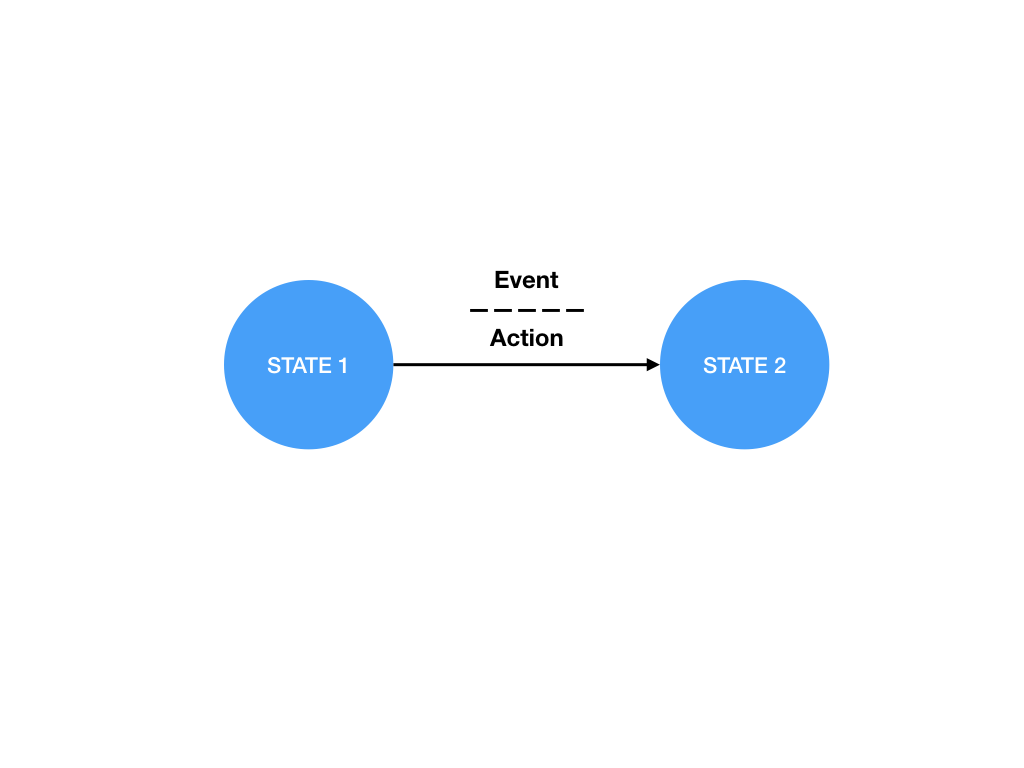
\includegraphics[trim=2in 3in 2in 3in,clip,width=5in]{figures/generic-states.png}
\caption{A pair of generic states and a transition between them.}
\label{fig:state.machine}
\end{figure}

To give a concrete example, consider an alarm clock. Figure~\ref{fig:alarm.clock} shows a state machine for a typical alarm clock with a snooze option. Starting in the \verb|OFF| state, let's walk through the diagram. When the user sets an alarm, the system moves from \verb|OFF| to \verb|RUNNING|. While in the \verb|RUNNING| state, the system checks to see of the clock time has passed the alarm time. When it does, the system starts buzzing and changes to the \verb|ALARMING| state. While in the \verb|ALARMING| state, if the user presses the snooze button, it does two things: turns off the buzzer and starts a snooze timer. When in the \verb|SNOOZING| state, if the snooze timer expires, the system turns the buzzer back on and goes back to the \verb|ALARMING| state. In any state, the user can cancel the alarm, which takes the system back to the \verb|OFF| state.

\begin{figure}[htbp]
\centering
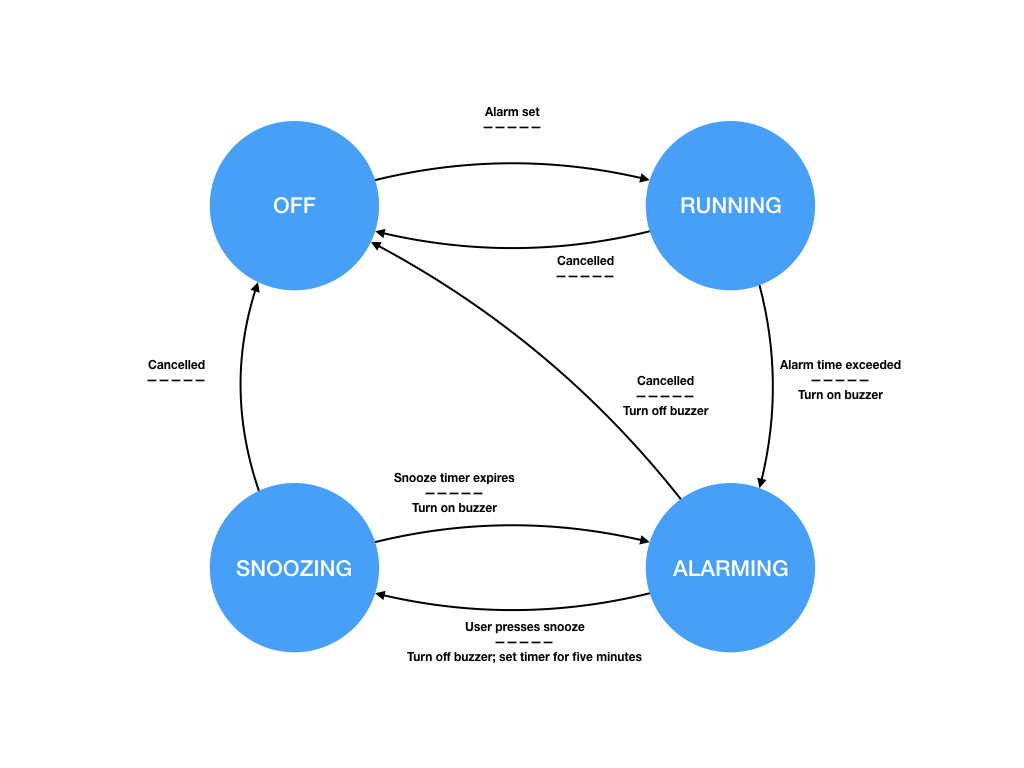
\includegraphics[trim=1.5in 1.5in 1.5in 1.5in,clip,width=6in]{figures/alarm-clock.png}
\caption{State machine for an alarm clock.}
\label{fig:alarm.clock}
\end{figure}

\subsubsection*{Coding a state machine}

We noted above that the system will transition from one state to another when a particular event occurs, for example the system goes from \verb|ALARMING| to \verb|SNOOZING| when the snooze button is pressed. Note, however, that not all events have meaning for every state. For example, in our alarm example, pressing the snooze button has no effect when the system is in the \verb|OFF| state.

Practically, what this means is that the system only needs to respond to a given event when it's in a state where that event is meaningful. The easiest way to manage this in code is to use a \emph{state variable} to track which state your system is in. To make the code more readable, you can use the \verb|enum| construction, which assigns numerical values to text descriptors, as follows:

\begin{verbatim}
    enum {OFF, RUNNING, ALARMING, SNOOZING};
    int currentState = OFF;
\end{verbatim}

Here we declare a set of states with four possible values. We then declare a specific variable, \verb|currentState|, which will be used to keep track of system’s current state. From there, it’s a matter of coding the state machine through conditional statements. For the event of pressing the snooze button, this might look something like the following in pseudo-code:

\begin{verbatim}
    begin HandleSnoozeButton
      if current state is ALARMING
        turn off the buzzer
        start a timer for five minutes
        change current state to SNOOZING
      else if in any other state
        ignore
      end if
    end
\end{verbatim}

Note that pressing the snooze button only has meaning when in the \verb|ALARMING| state -- in other states it is ignored. For practical reasons, it is often useful to use the \verb|switch| construct for actual code, but the syntax is a little complicated, so we won't spend time on that here (here's a \href{http://www.cplusplus.com/doc/tutorial/control/}{\underline{tutorial}}, if you're interested later). Just keep in mind that it's a convenient way to organize a bunch of \verb|if..else| statements if you ever get to that point in your project.

\section*{In the workshop}

\subsection*{Home alarm system}

Your challenge is to build and code a minimalist home alarm system. The system will need to allow activation and deactivation; sense an intruder; and sound an alarm if someone is detected. For each of these functions, you’ll use the following hardware and methods:

\begin{description}
\item[ Activation.] To activate your system, one will merely press a button. When activated, your system will turn on an LED that is pointed towards a photoresistor, which will be used for detecting an intruder -- a low-tech version of the laser systems seen in the movies.
\item[ Deactivation.] For deactivation, you'll need something more secure than a button. In this case you'll use an RFID reader to detect a specific tag. When deactivated the LED ``laser" will turn off.
\item[ Intrusion detection.] When the system is activated, if something comes between the LED and the photoresistor, occluding the ``laser", the system will alarm.
\item[ Alarming.] Alarming will consist a piezo buzzer that blares at 200 Hz. You must be able to deactivate the system with the RFID while it’s alarming.
\end{description}

A skeleton code will be provided that takes care of a lot of the tedious parts -- we want you to focus on implementation of the state machine.

\subsubsection*{Procedure}

\begin{enumerate}
\item \emph{Gently} place your RFID shield on your Arduino. Note that there are a lot of pins to get lined up, and it's easy to miss one and bend it. Don't worry too much -- pins can be unbent -- but the more careful you are, the better.
\item Consulting the LED/photoresisor circuits in Figure~\ref{fig:laser}, do the following. Don't get ahead of yourself here, do each step in order.
\begin{enumerate}
    \item Insert the photoresistor and LED into your breadboard about 3 - 4 cm apart. Gently bend the two so that the LED will shine directly on the photoresistor -- they should be about 1 cm from each other when you're all done -- you’ll want them close enough to get a good signal while still being able to pass a pencil or a finger between them without bumping either. Once you've arranged them, try not to move either component so that the measurements you are about to take will consistent for the rest of the lab.

\begin{figure}[htbp]
\begin{center}
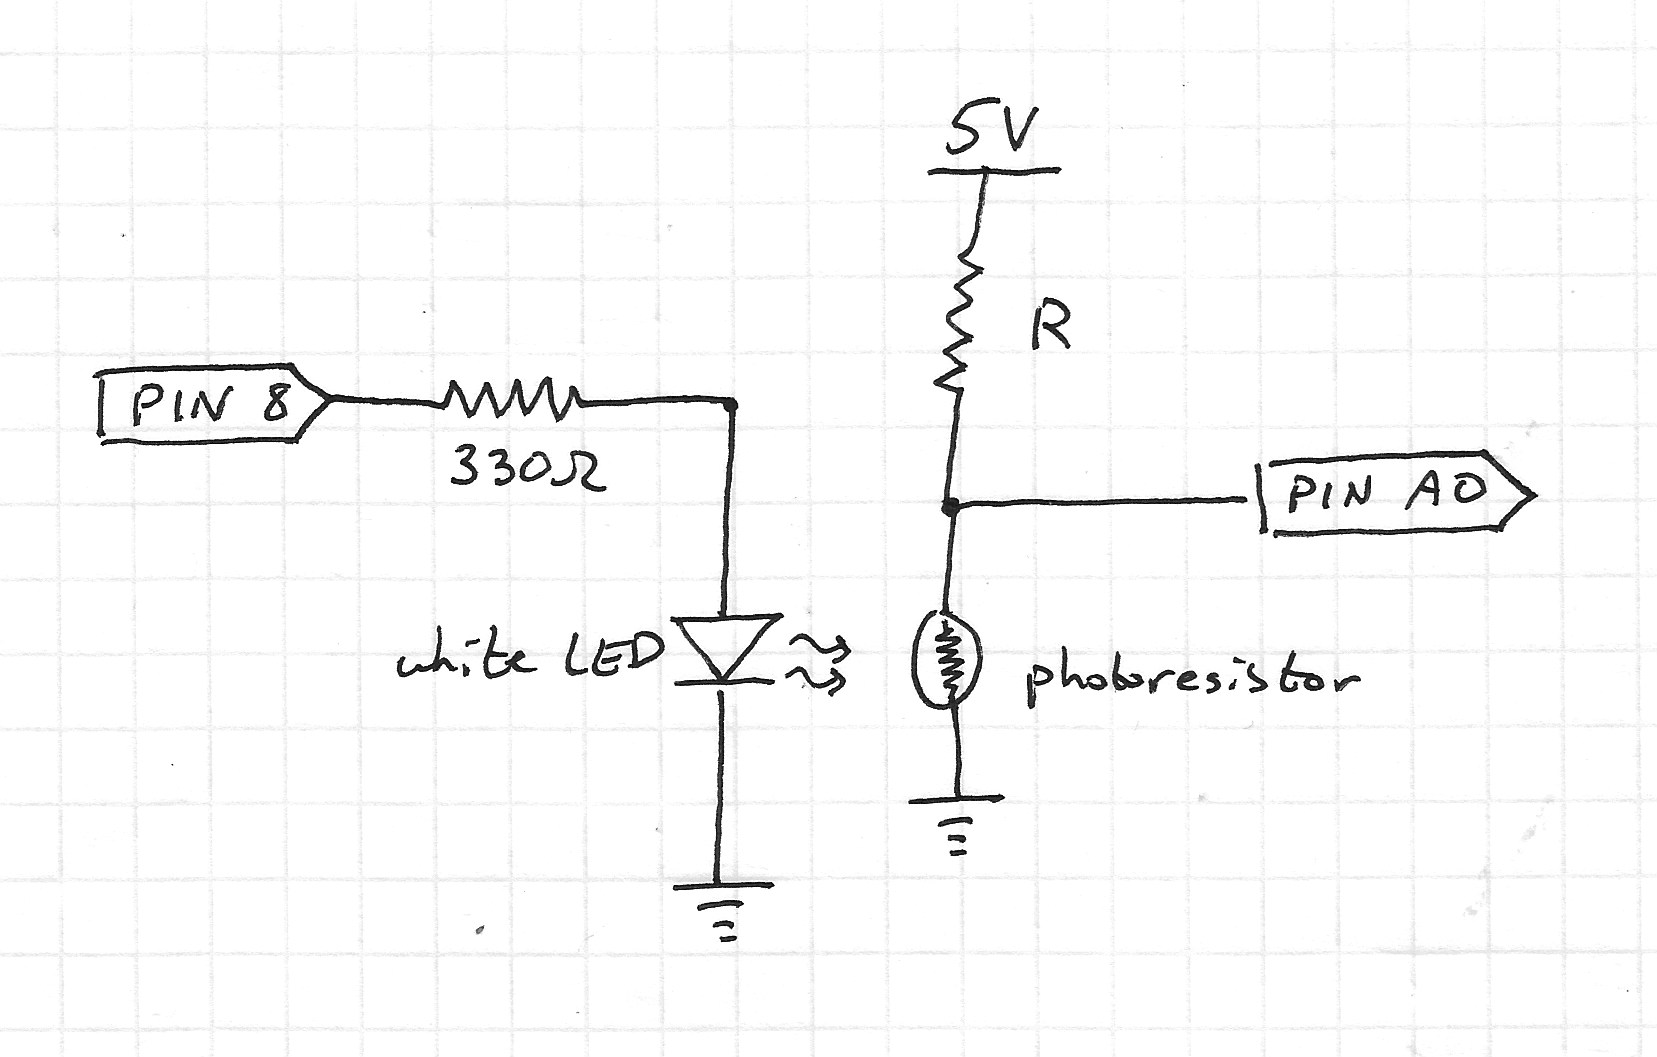
\includegraphics[width=4in]{figures/laser.png}
\caption{Circuits for the ``laser".}
\label{fig:laser}
\end{center}
\end{figure}

    \item Connect the LED as shown, but don't connect the photoresistor to anything yet. If you connect it to other components, you might not get good readings for the next steps.
    \item Using jumper wires (so you don’t disturb the photoresistor) and a \emph{digital multimeter} (DMM), measure and record the resistance of the photoresistor when the LED is on and when it is off. Record your values below.
    
    \vspace{0.25in}
    Resistance (LED on): \rule{2in}{0.4pt}

    \vspace{0.25in}
    Resistance (LED off): \rule{2in}{0.4pt}
    \vspace{0.25in}

    \item Choose a fixed resistor, $R$, with a value that is near the \emph{geometric mean}\footnote{It can be shown that doing so will give the largest voltage swing in your circuit, which makes it as sensitive as possible.} of the two values you measured above and complete the circuit.
    \item Use the example program \verb|AnalogReadSerial| (or write your own) to read the ADC at the junction and print it to the Serial Monitor every 500 ms. Run some tests to determine the ADC reading with the LED on and with it off. Choose a threshold that will serve to indicate that the beam is blocked -- that there is an intruder! Record your values below. How did you decide on a threshold value?

    \vspace{0.25in}
    ADC reading (LED on): \rule{2in}{0.4pt}

    \vspace{0.25in}
    ADC reading (LED off): \rule{2in}{0.4pt}

    \vspace{0.25in}
    Threshold ADC value: \rule{2in}{0.4pt}
    \vspace{0.25in}

\end{enumerate}
\item Build a button circuit on pin 7, except you don't need the pullup resistor. Instead, you'll use a nice feature of the Arduino, namely an internal pullup. To do so, you declare the pin mode as follows:

\begin{verbatim}
    pinMode(buttonPin, INPUT_PULLUP);
\end{verbatim}

This internal pullup has the same effect as the resistor you put in your breadboard, but without the hassle of extra wiring.

Note that you cannot use pins 2 and 3 for a button (as you did in the in-class tutorials) since they're used by the RFID shield.
\item Build the piezo ``buzzer" circuit in Figure~\ref{fig:piezo}. Note that the piezo circuit here is different from the one you built in the pre-lab. Specifically, the current draw of the piezo puts too much strain on a pin, so we'll have you build a high current circuit similar to the one you build for the motor.

\begin{figure}[htbp]
\begin{center}
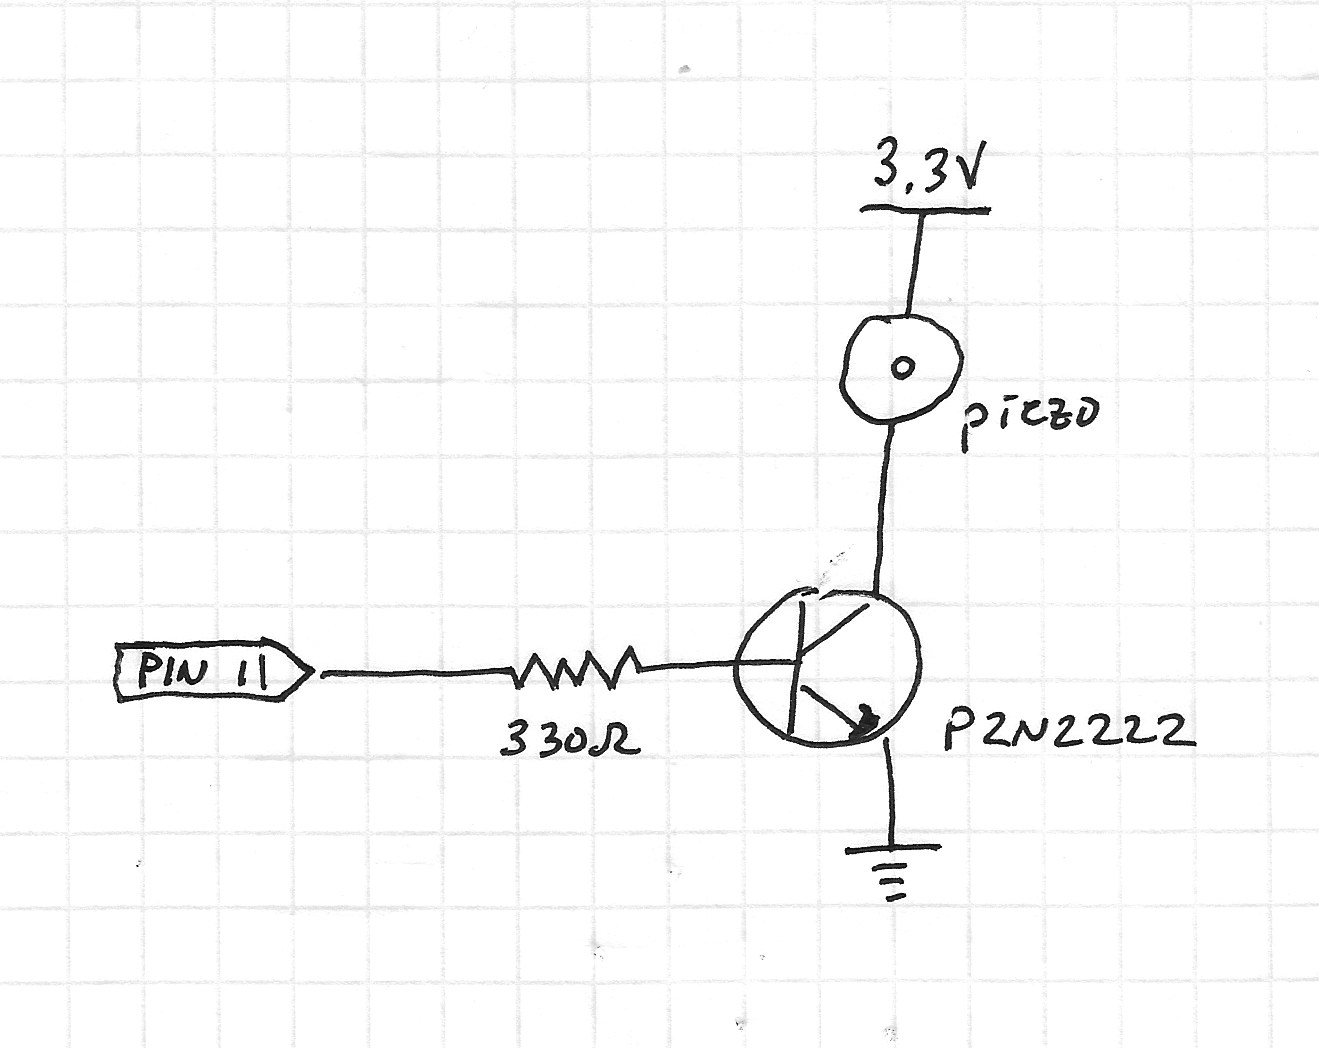
\includegraphics[width=4in]{figures/piezo.png}
\caption{Circuits for the piezo "buzzer".}
\label{fig:piezo}
\end{center}
\end{figure}

\item Grab the \verb|alarm_skeleton| code from \href{https://github.com/gcl8a/arduino.advanced}{\underline{github}}. Because of time constraints, we're not asking you to write code from scratch.
\item Grab the RFID library from \href{https://github.com/gcl8a/Adafruit-PN532}{\underline{github}}. Install it in the library folder in your sketchbook.
\item Though it's incomplete, upload the code to your Arduino and open the Serial Monitor. If all goes well, you should be able to place a tag near the RFID antenna and get a response. Pick which tag you want to be your "key" and note the 4-segment ID.
\item Go to the top of the code and change the \verb|targetID| to match the four values you just wrote down. Be sure to leave the \verb|0x| part in place -- this tells the Arduino that the numbers are in \emph{hexadecimal}, which is just a short hand for writing out bytes.
\item Re-upload the code, and now it should print ``\verb|Match!|" along with the tag ID. Once you've confirmed that the tag is correct, you should comment out all of the \verb|Serial.print| lines in \verb|CheckForRFID()| by placing a double slash, \verb|//|, at the beginning of each line. This will make the Serial Monitor much easier to read as we move forward.
\item Now you will fill in the missing parts of the state machine in the rest of the code. It may be helpful to put some \verb|Serial.print()| statements to help debug. Specifically, every time there is a transition, you should print something to the Serial Monitor. See \verb|HandleArmingButton()| in the code for an example.
\begin{enumerate}
    \item We've written the button checker function for you, but you need to finish the function for checking the laser. Your threshold from above will be used to check if the laser is broken. Note that you need to write it in proper event-driven form. Use the button checker as a template.
    \item We've started the button handler for you, but you'll have to fill in the actions. Note that we only explicitly address states that are specific to that event.
    \item You'll have to fill in the laser handler function. Don't forget to change the state when an event is handled!
    \item You'll also have to fill in the RFID handler. How many states does this handler apply to?
\end{enumerate}
\item Test your system. If it's not working, the first thing you'll want to do is determine if the problem is in hardware or software. To check if it's hardware, use known, working codes to test the components. You can also use a digital multimeter to check voltages, for example, at a pin. If you suspect that software is the problem, try putting \verb|Serial.print()| statements in useful places to help determine if the code is getting to where it should be.

Of course, you can always ask an instructor for some pointers.

\end{enumerate}

\textbf{Once you have a working system, show it to an instructor.}



\section*{Appendix: Arduino syntax}

The language used in the Arduino IDE is essentially \verb|C++|. For those who know \verb|C++|, you can use all of its constructs, including classes, structures, overloaded operators, virtual functions, and all kinds of other things that might not mean much to you if you haven't used them before.

No worries, though! You don't need to know all of the esoteric functionality of \verb|C++| to be able to write half-way decent programs in ``Arduino". At a minimum, you need to know the different datatypes, how to write a function, \verb|if..else| statements, \verb|for| and \verb|while| loops, and a few other things. Instead of re-hashing a lot of information that is out there, we'll simply point you to a \href{https://startingelectronics.org/software/arduino/learn-to-program-course/}{\underline{decent set of beginner tutorials}}. Look through them on your own time for hints and pointers on whatever you need or interests you.


\clearpage
\section*{Pre-lab}

\subsubsection*{Home alarm system}

\begin{enumerate}
\item In the workshop, you will be building a simplified home alarm system, but first, you’ll need to plan out the system using a state diagram. Your alarm system will have the following functionality:
\begin{itemize}
\item To arm the system, the user will push a button,
%\item When the system is armed, an indicator LED will light,
\item When the system is armed, an LED will shine on a photoresistor,
\item If an object comes between the LED and the photoresistor while the system is armed, an alarm will sound,
\item To disarm the system, regardless of whether or not it is alarming, the user will present a specific RFID tag,
\item When disarmed, the LED will turn off, and if the system is alarming, the sound will turn off, as well.
\end{itemize}

Draw out the state diagram for your alarm system. Be sure to include the states, events, and actions using the proper format shown in Figure~\ref{fig:state.machine}.
\vspace{2.5in}
\item Using pseudo-code, write out the handler function for responding to the correct RFID tag.

\end{enumerate}

\end{document}
